%%%%%%%%%%%%%%%%%%%%%%%%%%%%%%%%%%%%%%%%%%%%%%%%%%%%%%%%%%%%%%%%%%%%%%%%%%
\documentclass[twocolumns,10pt,a4j]{jarticle}
%%%%%%%%%%%%%%%%%%%%%%%%%%%%%%%%%%%%%%%%%%%%%%%%%%%%%%%%%%%%%%%%%%%%%%%%%%
\usepackage{amsmath}
\usepackage[dvipdfmx]{graphicx}% Include figure files
%\usepackage{txfonts}
\usepackage{setspace}
\usepackage{bm}% bold math
\usepackage{here}
\usepackage{array}
\usepackage[T1]{fontenc}
\usepackage{etoolbox}
\usepackage[top=10truemm,bottom=25truemm,left=25truemm,right=20truemm]{geometry}%余白
\usepackage{layout}
\usepackage{wrapfig}
\renewcommand{\abstractname}{} 
\renewcommand{\figurename}{\small{Fig.}}
\renewcommand{\thefootnote}{\fnsymbol{footnote}}
\renewcommand{\baselinestretch}{0.80}
\renewcommand{\thesection}{\arabic{section}.}
\usepackage{indentfirst}
\usepackage{otf}
%\usepackage{multicol}
\pagestyle{empty}
%%%%%%%%%%%%%%%%%%%%%%%%%%%%%%%%%%%%%%%%%%%%%%%%%%%%%%%%%%%%%%%%%%%%%%%%%%
\makeatletter%% プリアンブルで定義する場合は必須
\patchcmd{\maketitle}{\@fnsymbol}{\@alph}{}{}  % Footnote numbers from symbols to small letters
\long\def\@makecaption#1#2{% \@makecaption を再定義します
  \vskip\abovecaptionskip
  \iftdir\sbox\@tempboxa{#1\hskip1zw#2}%
  \else\sbox\@tempboxa{#1~ #2}% ここの : を ~ に変更する
  \fi
  \ifdim \wd\@tempboxa >\hsize% 
  \iftdir #1\hskip1zw#2\relax\par
  \else #1~ #2\relax\par\fi% ここの : を ~ に変更する
  \else
  \global \@minipagefalse
  \hbox to\hsize{\hfil\box\@tempboxa\hfil}% センタリング
  %   \hbox to\hsize{\box\@tempboxa\hfil}%      左詰め
  %   \hbox to\hsize{\hfil\box\@tempboxa}%      右詰め
  \fi
  \vskip\belowcaptionskip}

  \DeclareRobustCommand\cite{\unskip
  \@ifnextchar[{\@tempswatrue\@citex}{\@tempswafalse\@citex[]}}
  \def\@cite#1#2{$^{[\hbox{\scriptsize{#1\if@tempswa ,#2\fi}]}}$}
  \def\@biblabel#1{[#1]}
  \makeatother%% プリアンブルで定義する場合は必須
  \setlength{\columnsep}{8  truemm}
  \setlength{\linewidth}{81 truemm}
  %%%%%%%%%%%%%%%%%%%%%%%%%%%%%%%%%%%%%%%%%%%%%%%%%%%%%%%%%%%%%%%%%%%%%%
  \title{\Large 希薄系でのマイクロスイマーのダイナミクス\vspace{-3truemm}}
  \author{\large 化学プロセス工学コース 移動現象論分野 荊尾太雅\vspace{-10zh}}
  \date{}
  %%%%%%%%%%%%%%%%%%%%%%%%%%%%%%%%%%%%%%%%%%%%%%%%%%%%%%%%%%%%%%%%%%%%%%
  \begin{document}

  %% start abstract

  \twocolumn[
    \maketitle\thispagestyle{empty}
    \vspace{-10truemm}
    \begin{quote}
      \normalsize
マイクロスイマーとは,バクテリアのように粘性流体中を自己推進する微小な物体の総称である.
工学的にも応用性に富んでいるが,それらの集団運動を予測し制御するためには複雑な流体力学的相互作用を考慮する必要があり,未だに理解が進んでいない.
本研究ではsquirmerモデルを用いた直接数値計算を行い,希薄系でのbottom heavyな性質を付加したマイクロスイマーの挙動を調べた.
    \end{quote}
  ]

  %% end abstract
  %% start 1.緒言

  \noindent
  \textbf{\large 1.緒言}
  \par
マイクロスイマーの拘束空間内における集団的な動的挙動を理解することは,バイオフィルムの形成の説明や標的薬物送達システムの設計などの工学的な用途に有用である.
本研究では,直接数値計算を用いて,希薄系における,重心が中心からずれたbottom heavyな性質を持つマイクロスイマーの挙動を調べることを目的とした.

  %% end 1.
  %% start 2.計算手法

  \noindent
  \textbf{\large 2.計算手法}
  \par
マイクロスイマーのモデルとして,squirmerモデルを採用した.
このモデルでは,粒子表面において粒子と流体の速度差が式\eqref{boundary_I}で表される境界条件を用いる\cite{1}.

  \vspace{-3truemm}
    \begin{equation}
      \boldsymbol{u}^s = B_1 \left( \sin{\theta} + \frac{\alpha}{2} \sin{2\theta} \right) \hat{\boldsymbol{\theta}}
      \label{boundary_I}
    \end{equation}
  \vspace{-4truemm}

  \noindent
ここで,$\boldsymbol{u}^s$はスイマー表面の流れ場,$B_1$はフーリエ級数の係数第1項,$\alpha$はスイマーのタイプを与える定数,
$\theta$は動径ベクトルと推進方向との間の極角,$\hat{\boldsymbol{\theta}}$は単位極角ベクトルである.
$\alpha<0$では推進方向に伸張流場を生成するPusher型,
$\alpha=0$で潜在的な流れ場で泳ぐNeutral型,
$\alpha>0$で推進方向に収縮流場を生成するPuller型を示す.
直接数値計算は,squirmerモデルをSPMに組み込んで行った.
SPMは流体力学を用いた固体/流体2相ダイナミクス問題の効率的な計算方法である\cite{2}.
流体の支配方程式として非圧縮性流体におけるNavier-Stokes方程式\eqref{Navier_Stokes}を用い,
スイマーの時間発展はNewton-Euler方程式\eqref{Newton_Euler}で与えた.

\par
1.Navier-Stokes方程式\\
  \vspace{-3truemm}
  \small
  \begin{equation}
    \begin{split}
      \boldsymbol{\nabla}\cdot\boldsymbol{u} &= 0 \\
      \rho_\mathrm{f} \left(\partial_\mathrm{t} + \boldsymbol{u} \cdot \boldsymbol{\nabla} \right) \boldsymbol{u} &= \boldsymbol{\nabla} \cdot \boldsymbol{\sigma} + \rho_\mathrm{f} \left( \phi \boldsymbol{f}_\mathrm{p} + \boldsymbol{f}_\mathrm{sq} + \boldsymbol{f}^\mathrm{s} \right)
    \end{split}
    \label{Navier_Stokes}
  \end{equation}
  \normalsize
  \vspace{-4truemm}

  \noindent
ここで,$t$は時間,$\boldsymbol{u}$は全速度場,$\rho_\mathrm{f}$は流体の質量密度,$\boldsymbol{\sigma}$は流体の応力テンソル,
$\phi$は[0,1]の値を連続的に持つ界面関数,$\phi \boldsymbol{f}_\mathrm{p}$は粒子の剛直性を保証する体積力,
$\boldsymbol{f}_\mathrm{sq}$はスイマーの泳動による力,
$\boldsymbol{f}^\mathrm{s}$は式\eqref{zigzag_flow}のように表される速度を流体に生じさせる外力である.
  \par
  \vspace{-6truemm}
  \small
  \begin{equation}
    v_x(y) =
    \begin{cases}
      \dot{\gamma} (-y - L_y/2) & (-L_y/2 < y \le -L_y/4) \\
      \dot{\gamma} y            & (-L_y/4 < y \le L_y/4) \\
      \dot{\gamma} (-y + L_y/2) & (L_y/4 < y \le L_y/2)\\
    \end{cases}
    \label{zigzag_flow}
  \end{equation}
  \normalsize
  \vspace{-4truemm}

  \noindent
 ここで,$\dot{\gamma}$はせん断速度,$y$は系のy座標,$L_y$は系のy軸方向の大きさである.

  \par
2.Newton-Euler方程式\\
  \vspace{-6truemm}
  \begin{equation}
    \begin{split}
      \dot{\boldsymbol{R}}_i = \boldsymbol{V}_i &, \quad \boldsymbol{\dot{Q_i}} = \mathrm{skew} (\boldsymbol{\Omega_i}) \cdot \boldsymbol{Q_i} \\
      M_p \dot{\boldsymbol{V}_i} = \boldsymbol{F}_i^\mathrm{H} &, \quad
      \boldsymbol{I}_p \cdot \dot{\boldsymbol{\Omega}_i} = \boldsymbol{N}_i^\mathrm{H} + \boldsymbol{N}_i^\mathrm{b.h.}
    \end{split}
    \label{Newton_Euler}
  \end{equation}
  \vspace{-4truemm}

  \noindent
ここでスイマー$i$について,$\boldsymbol{R}_i$は位置,$\boldsymbol{V}_i$は速度,
$\boldsymbol{Q_i}$は回転行列,$\boldsymbol{\Omega}_i$は角速度,
$\mathrm{skew} (\boldsymbol{\Omega_i})$は$\boldsymbol{\Omega}_i$の交代行列を示す.
$M_\mathrm{p}$と$\boldsymbol{I}_\mathrm{p}$はそれぞれスイマーの質量と慣性モーメントを表す.$\boldsymbol{F}_i^\mathrm{H}$は流体から受ける力,
$\boldsymbol{N}_i^\mathrm{H}$は流体から受けるトルクである.
球形粒子の場合$N^\mathrm{H}$は式\eqref{nh}で表される.
  \vspace{-3truemm}
  \begin{equation}
    \boldsymbol{N^\mathrm{H}} = 4 \pi \mu a^3 \dot{\gamma}
    \label{nh}
  \end{equation}
  \vspace{-6truemm}

\noindent
ここで,$\mu$は流体の粘度,$a$は球形粒子の半径,$\dot{\gamma}$はせん断速度である.
$\boldsymbol{N}_i^\mathrm{b.h.}$はbottom heavyな性質によって生じるトルクで,式\eqref{nbh}によって計算される\cite{3}.
ここで,$a$はスイマーの半径,$\rho$は流体の密度,$h$は球の中心と重心との距離,$\boldsymbol{e}$はスイマーの方向ベクトル,$\boldsymbol{g}$は重力である.
  \vspace{-3truemm}
  \begin{equation}
    \boldsymbol{N}^\mathrm{b.h.} = \frac{4}{3} \pi a^3 \rho h \boldsymbol{e} \times \boldsymbol{g}
    \label{nbh}
  \end{equation}
  \vspace{-4truemm}

  %% end 2.
  %% start 3.結果と考察

  \noindent
  {\bf \large 3.結果と考察}
  \par
直径$5\Delta$の一つのスイマーについて,$64\Delta \times 128\Delta \times 64\Delta$の矩形システムでシミュレーションを行った.
このシステムでは,y軸方向に重力がかかり,x軸方向にせん断がかかっている.
ここで,$\Delta$は格子間隔と単位長さである.
通常の球形粒子とPusher型/Puller型の3種について,せん断の大きさと粒子の進行方向の関係を表したものが図である.
  \vspace{-3truemm}
  \begin{figure}[h]
    \begin{tabular}{cc}
      \hspace{-3truemm}
      \begin{minipage}[t]{0.44\hsize}
        \centering
        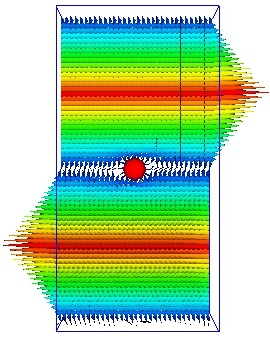
\includegraphics[width=30truemm]{./images/zig_zag.jpg}
        \vspace{-4truemm}
        \hspace{-2truemm}
        \caption{Simulation snapshot}
        \label{zigzag_image}
      \end{minipage}

      % \hspace{2mm}
      % \vspace{-2mm}
      \begin{minipage}[t]{0.44\hsize}
        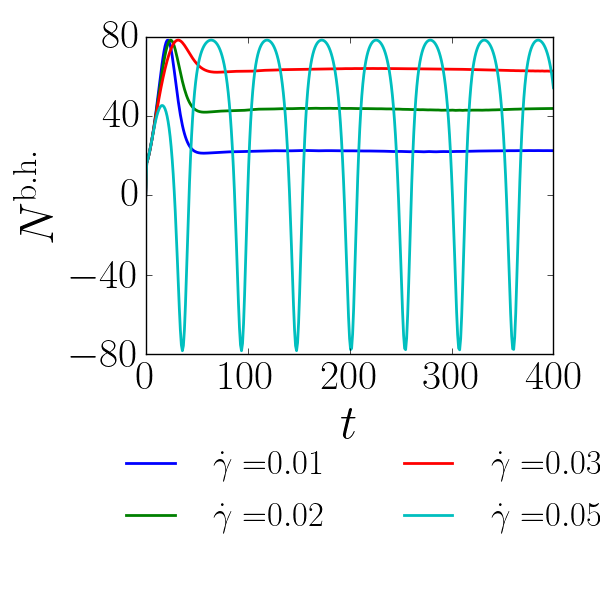
\includegraphics[width=37truemm]{./images/00.png}
        \vspace{-10truemm}
        \caption{Time evolution of bottom heaviness torque}
        \label{wave}
      \end{minipage}
      % \vspace{-1mm}
    \end{tabular}
  \end{figure}

  \noindent
ここで,$\dot{\gamma}$はせん断速度を表す.
球形粒子の場合,式\eqref{nh}と\eqref{nbh}が等しいとして求まる$\dot{\gamma}$と,シミュレーション結果がよく一致していることが確認できた.
bottom heavyな性質から生じるトルクの項を新たに追加することで,系にかかる重力の逆向きに進もうとするスイマーの性質を再現することができた.


  %% end 3.
  %% start 4.結言

  \noindent
  \textbf{\large 4.結言}
  \par
マイクロスイマーのモデルにsquirmerモデルを採用し,平行壁に挟まれた矩形システムの中でマイクロスイマー2成分系の局所密度の時間発展の解析を行った.
その結果,Puller型の分率が多いほどシステム内における疎密波の形成傾向が強まることを定量的に示した.
  \vspace{-7.5truemm}

  %% end 4.
  %% start 参考文献

  \renewcommand{\refname}{\normalsize 参考文献\vspace{-3truemm}}
  \begin{thebibliography}{9}
  %
  \bibitem{1}
    N. Oyama,博士論文,(2017).\\
  %
  \vspace{-7truemm}
  %
  \bibitem{2}
    Y. Nakayama,K. Kim,and R. Yamamoto,\textit{The European Physical Journal E},\textbf{26},361-368 (2008).\\
  %
  \vspace{-7truemm}
  %
  \bibitem{3}
    hoge
  \end{thebibliography}

  %% end 参考文献
  %% satrt 締め

  % \vspace{-7truemm}
  \centering
  \underline{指導教員名\hspace{10truemm} 山本 量一 \hspace{20truemm} 印}

  %% end 締め

\end{document}
